\documentclass[12pt,a4paper]{article}

\renewcommand*\contentsname{Sadržaj}
\renewcommand{\figurename}{Slika}
\renewcommand{\tablename}{Tabela}
\renewcommand\refname{Reference}
\renewcommand{\arraystretch}{1.25}

\usepackage[margin=0.85in]{geometry}
\usepackage{graphicx}
\usepackage{float}
\usepackage{listings}
\usepackage{multirow}
\usepackage[table]{xcolor}
\usepackage{colortbl}
\usepackage{color}
\usepackage{hyperref}
\usepackage{ctable}
\usepackage{array}
\usepackage{hhline}
\usepackage{caption}
\usepackage{amsfonts}
\usepackage{flowchart}
\usepackage{algpseudocode}
\usepackage[shortlabels]{enumitem}
\usepackage{algorithm2e}
\renewcommand{\algorithmcfname}{Algoritam}
\usetikzlibrary{arrows}

\lstloadlanguages{C,C++,csh,Java}

\definecolor{red}{rgb}{0.6,0,0} 
\definecolor{blue}{rgb}{0,0,0.6}
\definecolor{green}{rgb}{0,0.8,0}
\definecolor{cyan}{rgb}{0.0,0.6,0.6}
\definecolor{magnolia}{rgb}{0.97, 0.96, 1.0}
\definecolor{colora}{rgb}{0.67, 0.8, 0.94}
\definecolor{colorb}{rgb}{0.67, 0.94, 0.82}
\definecolor{colord}{rgb}{0.67, 0.9, 0.93}
\definecolor{colore}{rgb}{0.6, 0.73, 0.89}
\definecolor{colorf}{rgb}{0.61, 0.87, 1.0}
\definecolor{grey}{rgb}{0.75, 0.75, 0.75}

\lstset{
language=csh,
basicstyle=\footnotesize\ttfamily,
numbers=left,
numberstyle=\tiny,
numbersep=5pt,
tabsize=2,
extendedchars=true,
breaklines=true,
frame=b,
stringstyle=\color{blue}\ttfamily,
showspaces=false,
showtabs=false,
xleftmargin=17pt,
framexleftmargin=17pt,
framexrightmargin=5pt,
framexbottommargin=4pt,
commentstyle=\color{green},
morecomment=[l]{//}, %use comment-line-style!
morecomment=[s]{/*}{*/}, %for multiline comments
showstringspaces=false,
morekeywords={ abstract, event, new, struct,
as, explicit, null, switch,
base, extern, object, this,
bool, false, operator, throw,
break, finally, out, true,
byte, fixed, override, try,
case, float, params, typeof,
catch, for, private, uint,
char, foreach, protected, ulong,
checked, goto, public, unchecked,
class, if, readonly, unsafe,
const, implicit, ref, ushort,
continue, in, return, using,
decimal, int, sbyte, virtual,
default, interface, sealed, volatile,
delegate, internal, short, void,
do, is, sizeof, while,
double, lock, stackalloc,
else, long, static,
enum, namespace, string},
keywordstyle=\color{cyan},
identifierstyle=\color{red},
backgroundcolor=\color{magnolia},
}

\DeclareCaptionFont{white}{\color{white}}
\DeclareCaptionFormat{listing}{\colorbox{blue}{\parbox{\textwidth}{\hspace{15pt}#1#2#3}}}
\captionsetup[lstlisting]{format=listing,labelfont=white,textfont=white, singlelinecheck=false, margin=0pt, font={bf,footnotesize}}

\newcolumntype{a}{>{\columncolor{colora}}c}
\newcolumntype{b}{>{\columncolor{colorb}}c}
\newcolumntype{d}{>{\columncolor{colord}}c}
\newcolumntype{e}{>{\columncolor{colore}}c}
\newcolumntype{f}{>{\columncolor{colorf}}c}
\newcolumntype{P}[1]{>{\centering\arraybackslash}p{#1}}
\newcolumntype{?}{!{\vrule width 1pt}}

\begin{document}

\begin{titlepage}
	\centering
	{\scshape Univerzitet u Sarajevu \par}
	{\scshape Elektrotehnički Fakultet \par}
	{\scshape Odsjek za Računarstvo i Informatiku \par}
	\vspace{2cm}
	{\Large\scshape Biomedicinski Signali i Sistemi\par}
	\vspace{2.5cm}
	{\huge\bfseries Seminarski Rad\par}
	\vspace{2.5cm}
	{\huge\bfseries Aritmija i hipertenzija te njihov utjecaj na EKG signale\par}
	\vspace{2.5cm}
	\Large Student: \par
	{\Large\itshape \textsc{Krupalija} Ehlimana, 1431/17461\par}
	\vfill
	Predmetni nastavnik:\par
	v. prof. dr. \textsc{Dušanka Bošković}, dipl. ing. el.
	\vfill
	{\large Juli, 2019\par}
\end{titlepage}

\pagenumbering{gobble}

\tableofcontents

\newpage

\pagenumbering{arabic}

\section{Uvod}

\quad Elektrokardiogram (EKG) je graf koji prikazuje promjenu u električnoj aktivnosti srca kroz vrijeme. Korištenjem ove tehnologije moguće je analizirati rad srca, budući da tokom različitih faza rada srca (sistole i dijastole) dolazi do pojave različitih vrijednosti napona koje je moguće izmjeriti te na taj način detektovati karakteristike rada srca (tzv. PQRS kompleks prikazuje se na EKG signalu te je njegovom analizom moguće doći do velikog broja podataka koji mogu biti korisni u detektovanju simptoma te dijagnostici različitih stanja i bolesti). \\

Jedan veoma čest i rasprostranjen poremećaj srca je aritmija, te je vršenje dijagnosticiranja ovog poremećaja jednostavno i brzo, budući da se na jednom EKG signalu može vrlo lako uočiti nepravilnost u radu srca. Jedan veoma čest poremećaj usko vezan s radom srca je visok krvni pritisak, koji u različitim slučajevima može dovesti do različitih poremećaja u radu srca, koje je također veoma lako uočiti na EKG signalu. Budući da je vršenje elektrokardiografije bezbolno i brzo, korištenje ove tehnike za dijagnosticiranje i analizu veoma je često. \\

Pojava velikog broja softverskih alata za prikupljanje i analizu EKG signala olakšava analizu svih ovih podataka. Postoji veliki broj baza podataka u kojima se nalaze sortirani EKG signali pacijenata s različitim poremećajima, među kojima važno mjesto zauzimaju baze podataka pacijenata koji imaju aritmiju i hipertenziju (visok krvni pritisak). Iz tog razloga, analizom ovakvih EKG signala moguće je doći do velikog broja informacija koje mogu pomoći pri dijagnosticiranju ovih bolesti veoma rano nakon njihovog nastanka kako bi se mogle tretirati i uspješno kontrolisati (te i izliječiti). \\

U ovom radu biti će dat opis aritmije i visokog krvnog pritiska kao poremećaja koji se mogu dovesti u vezu s EKG signalima, te će biti izvršena analiza signala iz baza podataka pacijenata s ovim poremećajima koristeći alate razvijene u programskom jeziku \textit{Python}, nakon čega će se ova dva poremećaja pokušati dovesti u vezu te se donijeti zaključci o zajedničkim osobinama EKG signala iz ovih baza podataka.

\newpage

\section{Poremećaji koji dovode do promjene EKG signala}

\subsection{Aritmija}

\quad Normalan rad srca karakteriše stabilan ritam rada - srce koje pravilno radi, pumpa krv u pravilnim vremenskim razmacima te je ritam srca pravilan i ujednačen. U slučaju pravilnog rada srca, na EKG snimku moguće je vidjeti pravilan razmak između PQRS kompleksa - depolarizacija pretkomora i komora, grčenje srčanog mišića, pumpanje krvi te polarizacija i opuštanje srčanog mišića dešavaju se u pravilnim vremenskim razmacima. Ovi vremenski razmaci mogu varirati u rasponu od maksimalno $\delta$ = 0.16 sekundi. EKG snimak pacijenata koji nemaju aritmiju sastoji se od 60 do 100 PQRS kompleksa po minuti (mada se granica tolerancije u nekim slučajevima može spustiti i do 50 bpm). \cite{arrhythmia-book} \\

Tipičan EKG snimak pacijenta čije srce karakteriše pravilan rad moguće je vidjeti na Slici \ref{s1}. Vidljivo je da se otkucaji srca javljaju u pravilnim razmacima, bez većih fluktuacija koje bi ukazivale na neku bolest poput aritmije.

\begin{figure}[H]
\center
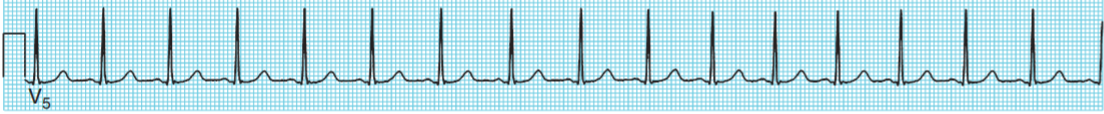
\includegraphics[scale=0.7]{../res/s1.PNG}
\caption{Prikaz EKG signala pacijenta koji nema srčanih problema}
\label{s1}
\end{figure}

Ukoliko srce pacijenta kuca sporije od 60 (odnosno 50), ili brže od 100 puta u minuti, te ukoliko su varijacije između srednje veličine razmaka između pojedinačnih otkucaja (PQRS kompleksa) veće od 0.16 sekundi, pacijentu se dijagnosticira stanje koje se naziva \textbf{aritmija}. Aritmija zapravo označava zdravstveno stanje u kojem srce nije u mogućnosti da ispravno kontroliše svoj rad, te se kao posljedica faze kontrakcija i opuštanja dešavaju u nepravilnim razmacima, te ih zbog toga ima ili manje, ili više nego što bi trebalo kako bi srčani sistem ispravno funkcionisao, te kako bi količina krvi u krvotoku bila u dozvoljenim granicama. \cite{arrhythmia-basics} \\ 

Tipičan EKG snimak pacijenta čije srce karakteriše nepravilan rad moguće je vidjeti na Slici \ref{s2}. Vidljivo je da se otkucaji srca javljaju u izrazito nepravilnim razmacima, s velikim fluktuacijama koje nedvosmisleno vode do zaključka da pacijent boluje od aritmije.

\begin{figure}[H]
\center
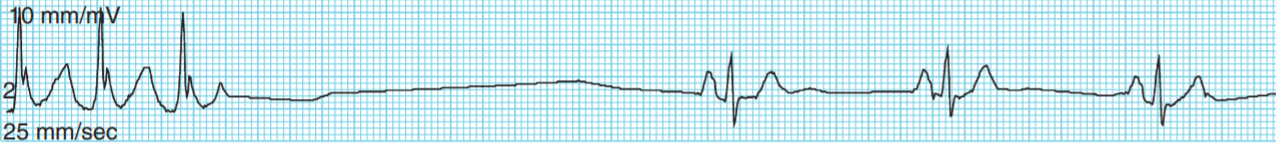
\includegraphics[scale=0.6]{../res/s2.PNG}
\caption{Prikaz EKG signala pacijenta koji boluje od aritmije}
\label{s2}
\end{figure}

\quad Postoje dva glavna uzroka aritmije:

\begin{enumerate}

\item \textit{Nepravilan rad sinusnog čvora}, tzv. \textit{pacemaker}-a srca, zbog kojeg srce nepravilno pumpa krv te se depolarizacija ne dešava uvijek u isto vrijeme, već u nepravilnim razmacima. Ovakav tip aritmije naziva se \textbf{sinusnom aritmijom}, te je karakterističan za sportiste, čiji metabolizam i način života dovode do poremećaja u funkcijama sinusnog čvora, zbog čega se javlja nepravilan rad srca. Tipičan primjer ovog tipa aritmije može se vidjeti na Slici \ref{s3}.

\begin{figure}[H]
\center
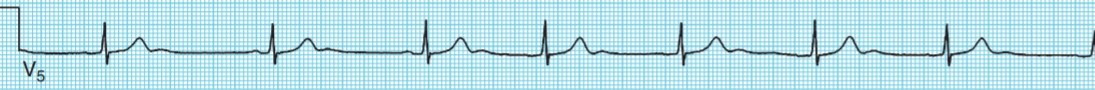
\includegraphics[scale=0.7]{../res/s3.PNG}
\caption{Prikaz EKG signala pacijenta koji boluje od sinusne aritmije}
\label{s3}
\end{figure}

\item \textit{Nepravilna električna provodnost}, koja se odnosi na nakupljanje električnog naboja koji dovodi do pojave lažne depolarizacije samo trenutak nakon što se završi jedan ciklus rada srca (otkucaj), što za posljedicu ima novi ciklus (novi otkucaj) prije nego prođe faza mirovanja. Ovakav tip aritmije karakterističan je za pacijente koji koriste opojna sredstva ili neku drugu vrstu stimulanata što dovodi do poremećaja u električni sredini cijelog tijela, te što za posljedicu ima i poremećaj rada srca. Tipičan primjer ovog tipa aritmije može se vidjeti na Slici \ref{s4}.

\begin{figure}[H]
\center
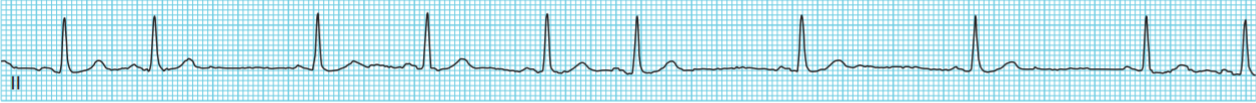
\includegraphics[scale=0.6]{../res/s4.PNG}
\caption{Prikaz EKG signala pacijenta koji boluje od ventrikularne aritmije}
\label{s4}
\end{figure}

\end{enumerate}

\subsection{Poremećaji krvnog pritiska}

\quad Vrijednost krvnog pritiska u arterijama stalno se mijenja, jer krv nije statična komponenta u tijelu, već konstantno protiče kroz krvne žile (prosječan protok krvi kroz arterije mjeri se u kubnim centimetrima i ovisi od veličine arterije i njenog položaja u tijelu). \cite{blood-pressure}
Postoje dvije karakteristične vrijednosti krvnog pritiska:

\begin{enumerate}

\item \textit{Sistolni krvni pritisak}, koji predstavlja maksimalnu vrijednost krvnog pritiska koja se pojavljuje u fazi kontrakcije srca (tokom sistole);

\item \textit{Dijastolni krvni pritisak}, koji predstavlja minimalnu vrijednost krvnog pritiska koja se pojavljuje u fazi opuštanja srca (tokom dijastole).

\end{enumerate}

Normalan krvni pritisak iznosi oko 120 mmHg (sistolni krvni pritisak) i 80 mmHg (dijastolni krvni pritisak), što se jednostavnije označava kao 120/80. Postoji više vrsta poremećaja krvnog pritiska, poput npr. malog raspona između sistolnog i dijastolnog pritiska (što može simptom velikog broja stanja, od nesvjestice do problema s radom srca), širokog raspona pulsa (što može biti simptom problema u radu aorte ili drugih arterija u tijelu) i sl. \cite{wide-pulse-pressure} \\

Dva najčešća poremećaja krvnog pritiska su \textbf{hipotenzija} (nizak krvni pritisak) i \textbf{hipertenzija} (visok krvni pritisak). Niskim, odnosno visokim krvnim pritiskom smatraju se sve vrijednosti krvnog pritiska koje su manje ili jednake, odnosno veće ili jednake tipičnim vrijednostima (npr. visokim krvnim pritiskom smatra se i krvni pritisak 140/110 i 130/80, pri čemu u prvom slučaju postoji poremećaj uskog raspona pulsa, dok u drugom slučaju postoji poremećaj širokog raspona pulsa). Glavna razlika između ova dva poremećaja, kada su u pitanju analize EKG signale, predstavljaju posljedice ovih stanja na rad srca. \\

U slučaju niskog krvnog pritiska, može doći do nesvjestice te težih problema koji mogu biti opasni po život, no nizak krvni pritisak ne može biti uzrok oštećenja srca niti srčanih funkcija - naprotiv, nizak krvni pritisak je često simptom disfunkcije srca (odnosno, srce koje slabije radi uzrokuje slabiji protok krvi kroz arterije, te je samim tim i krvni pritisak niži) \cite{low-pressure}. S druge strane, loše ili nikakvo tretiranje visokog krvnog pritiska može dovesti do oštećenja ne samo funkcija arterija, već i kompletnog srca. Iz tog razloga mnogo je važnije vršiti analizu EKG signala kod pacijenata s visokim krvnim pritiskom kako bi se utvrdilo da li ima poremećaja u ritmu rada srca, dok su EKG signali pacijenata s niskim krvnim pritiskom karakterisani manjim amplitudama, no bez tendencije promjena u samim fazama rada srca kroz vrijeme. \cite{high-pressure} \\

Na Slici \ref{s5} prikazan je EKG signal pacijenta koji duži vremenski period boluje od visokog krvnog pritiska, bez korištenja lijekova za kontrolisanje ovog stanja. Na slici je vidljivo da je na samom grafu veoma teško utvrditi ikakvu pravilnost u ritmu rada srca, da PQRS kompleksi imaju različite oblike u svakom ciklusu rada srca (odnosno, da grčenje i opuštanje srca imaju različita trajanja i intenzitete), na osnovu čega je veoma lako zaključiti da visok krvni pritisak nije stanje koje se ne bi trebalo tretirati, jer može dovesti do velikog broja poremećaja srca, kao i drugih dijelova organizma. \cite{pressure-ECG}

\begin{figure}[H]
\center
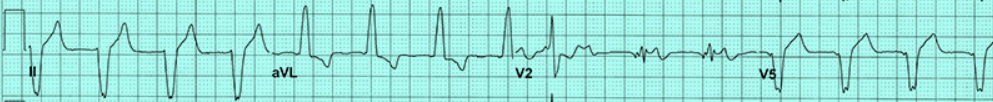
\includegraphics[scale=0.7]{../res/s5.PNG}
\caption{Prikaz EKG signala pacijenta koji boluje od hipertenzije \cite{pressure-ECG}}
\label{s5}
\end{figure}

\newpage

\section{Analiza EKG signala}

\quad Za analizu EKG signala pacijenata s prethodno opisanim vrstama poremećaja (aritmija i visok krvni pritisak)\footnote{Cijeli kod dostupan je na sljedećem linku: \url{https://github.com/ehlymana/ECGAnalysis}.} biti će korištene sljedeće PhysioNet baze podataka \cite{physionet}:

\begin{itemize}
\renewcommand\labelitemi{-}

\item \textit{Baza podataka za pacijente s aritmijom}: \href{https://physionet.org/physiobank/database/mitdb/}{MIT-BIH Arrhythmia Database} \cite{mit-bih};

\item \textit{Baza podataka za pacijente s visokim krvnim pritiskom}\footnote{Budući da svi signali iz ove baze podataka zauzimaju veliku količinu podataka (> 1 GB), isti nisu postavljeni u repozitorij projekta.}: \href{https://physionet.org/physiobank/database/shareedb/}{Smart Health for Assessing the Risk of Events via ECG (SHAREE) Database} \cite{sharee}.

\end{itemize}

Sadržaj repozitorija vidljiv je na Slici \ref{repository}. Za analizu EKG signala kreirana su četiri različita programska koda:

\begin{enumerate}

\item \texttt{download\_databases}: Služi za preuzimanje signala koje je potrebno analizirati iz zvaničnih PhysioNet baza podataka;

\item \texttt{heart\_rate\_analysis}: Služi za izračunavanje pojedinačnih te prosječnih brzina otkucaja srca ciljanih EKG signala, te za njihov prikaz na graficima u obliku funkcija i histograma;

\item \texttt{plot\_signals}: Služi za prikazivanje EKG signala iz baza podataka na graficima, pojedinačno ili kombinovano, u vremenu cijelog trajanja snimka ili samo u određenim trenucima;

\item \texttt{xqrs\_analysis}: Služi za izračunavanje širine QRS kompleksa svih EKG signala u bazama podataka te njihovo uspoređivanje.

\end{enumerate}

\begin{figure}[H]
\center
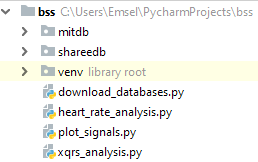
\includegraphics[scale=0.7]{../res/repository.PNG}
\caption{Sadržaj repozitorija programskog rješenja za analizu PhysioNet EKG signala}
\label{repository}
\end{figure}

\subsection{Preuzimanje signala iz ciljanih baza podataka}

\quad Biblioteka \texttt{wfdb} prilagođena je PhysioNet bazama podataka te omogućava ne samo jednostavnu analizu i prikaz podataka, već i preuzimanje sadržaja (što je mnogo teže uraditi koristeći direktno PhysioNet). U Listingu \ref{downloadlst} prikazan je način preuzimanja podataka iz ciljanih PhysioNet baza podataka - dovoljno je specificirati željeni direktorij u koji će svi signali biti preuzeti. Nakon pokretanja, korisnik dobiva informacije u konzoli kao što je prikazano na Slici \ref{download}. Važno je napomenuti da se MIT-BIH i SHAREE baze podataka razlikuju u mnogočemu, uključujući tip anotacija (MIT-BH: \texttt{atr}, SHAREE: \texttt{qrs}), no najistaknutija razlika je veličina podataka, zbog čega preuzimanje podataka iz MIT-BIH baze traje nekoliko sekundi, dok preuzimanje podataka iz SHAREE baze traje više od pola sata.

\begin{figure}
\captionof{lstlisting}{Preuzimanje traženih PhysioNet baza podataka}
\label{downloadlst}
\begin{lstlisting}[language=python]
import wfdb # for physionet tools
import os # for downloading samples from databases
from IPython.display import display # for displaying physionet libraries

if __name__ == '__main__':

    # Make download directories in your current working directory
    current_working_directory = os.getcwd()

    # the download directory for the arrhythmia database
    directory_database1 = os.path.join(current_working_directory, 'mitdb')

    # the download directory for the hypertension database
    directory_database2 = os.path.join(current_working_directory, 'shareedb')

    # Download all the WFDB content
    wfdb.dl_database('mitdb', dl_dir=directory_database1)
    wfdb.dl_database('shareedb', dl_dir=directory_database2)

    # Display the downloaded content in the folders
    display(os.listdir(directory_database1))
    display(os.listdir(directory_database2))
\end{lstlisting}
\end{figure}

\begin{figure}[H]
\center
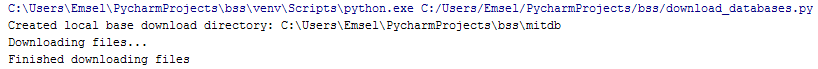
\includegraphics[scale=0.7]{../res/download.PNG}
\caption{Prikaz informacija o preuzimanju signala iz ciljanih baza podataka u konzoli}
\label{download}
\end{figure}

\subsection{Prikaz EKG signala}

\quad Biblioteka \texttt{wfdb} nudi i alate za vrlo jednostavan prikaz prethodno preuzetih EKG signala. Najvažnije funkcije koje se koriste za prikaz EKG signala su:

\begin{itemize}
\renewcommand\labelitemi{-}

\item \texttt{wfdb.plot\_items}, koja zahtijeva prethodno učitavanje signala koristeći funkciju \texttt{wfdb} \texttt{.rdrecord} te učitavanje anotacija za dati signal koristeći funkciju \texttt{wfdb.rdann}. Prikaz signala koristeći ovu funkciju moguć je od prvog do ciljanog trenutka (odnosno, nemoguće je prikazati signal počevši od nekog proizvoljnog trenutka, već je potrebno produžiti trajanje prikaza te izvršiti uvećavanje na grafiku);

\item \texttt{matplotlib.pyplot.plot}, koja se koristi za prikaz bilo kakvih signala na graficima, te biblioteka \texttt{wfdb} nudi i alate za pretvaranje signala u oblik pogodan za ovakav prikaz, koristeći funkciju \texttt{wfdb.rdsamp}. Na ovaj način moguće je jednostavno izbjeći ograničenja korištenja gotove funkcije za prikaz signala, te je tako moguće na jednom grafiku prikazati više EKG signala, u proizvoljnim bojama, te specificirajući željene početne i završne trenutke prikaza signala.

\end{itemize}

Korištenje \texttt{wfdb} funkcije za prikaz signala demonstrirano je u Listingu \ref{wfdb-plot}. Ukoliko se želi prikazati signal od početnog do ciljanog trenutka, ovakav prikaz dovoljan je da se dobiju sve neophodne informacije, kao što je prikazano na Slici \ref{plot-arrhythmia}, dok je u slučaju traženog prikaza od nekog drugog trenutka potrebno izvršiti manuelno uvećanje na dobivenom grafiku, kao što je prikazano na Slici \ref{plot-hypertension}. Za signal koji prikazuje hipertenziju ovakav prikaz je prijeko potreban, jer prikaz relevantnih informacija počinje neko vrijeme nakon početka snimka, te bi prikaz od početnog trenutka bio nerelevantan za sve analize i proučavanja. 

\begin{figure}
\captionof{lstlisting}{Prikaz EKG signala koristeći biblioteku \texttt{wfdb}}
\label{wfdb-plot}
\begin{lstlisting}[language=python]
    # Load record and annotation for the sample arrhythmia signal

    record_arrhythmia = wfdb.rdrecord('mitdb/100', sampfrom=0, sampto=4000)
    annotation_arrhyhthmia = wfdb.rdann('mitdb/100', 'atr', sampfrom=0, sampto=4000)

    # Plot signal

    wfdb.plot_items(signal=record_arrhythmia.p_signal, ann_samp=[annotation_arrhyhthmia.sample], title='MIT-BIH Record 100',
                    time_units='samples', figsize=(10, 4))

    # Load record and annotation for the sample hypertension signal

    record_hypertension = wfdb.rdrecord('shareedb/01911', sampfrom=0, sampto=104000)
    annotation_hypertension = wfdb.rdann('shareedb/01911', 'qrs', sampfrom=0, sampto=104000)

    # Plot signal

    wfdb.plot_items(signal=record_hypertension.p_signal, ann_samp=[annotation_hypertension.sample],
                    title='SHARE-EDB Record 01911',
                    time_units='samples', figsize=(10, 4))
\end{lstlisting}
\end{figure}

\begin{figure}[H]
\center
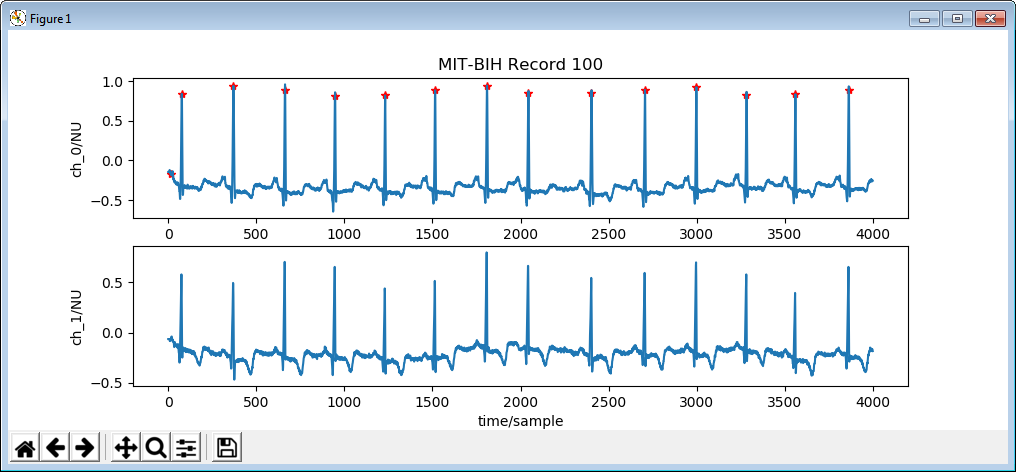
\includegraphics[scale=0.55]{../res/plot-mit.PNG}
\caption{Prikaz EKG signala iz MIT-BiH baze podataka koristeći biblioteku \texttt{wfdb}}
\label{plot-arrhythmia}
\end{figure}

\begin{figure}[H]
\center
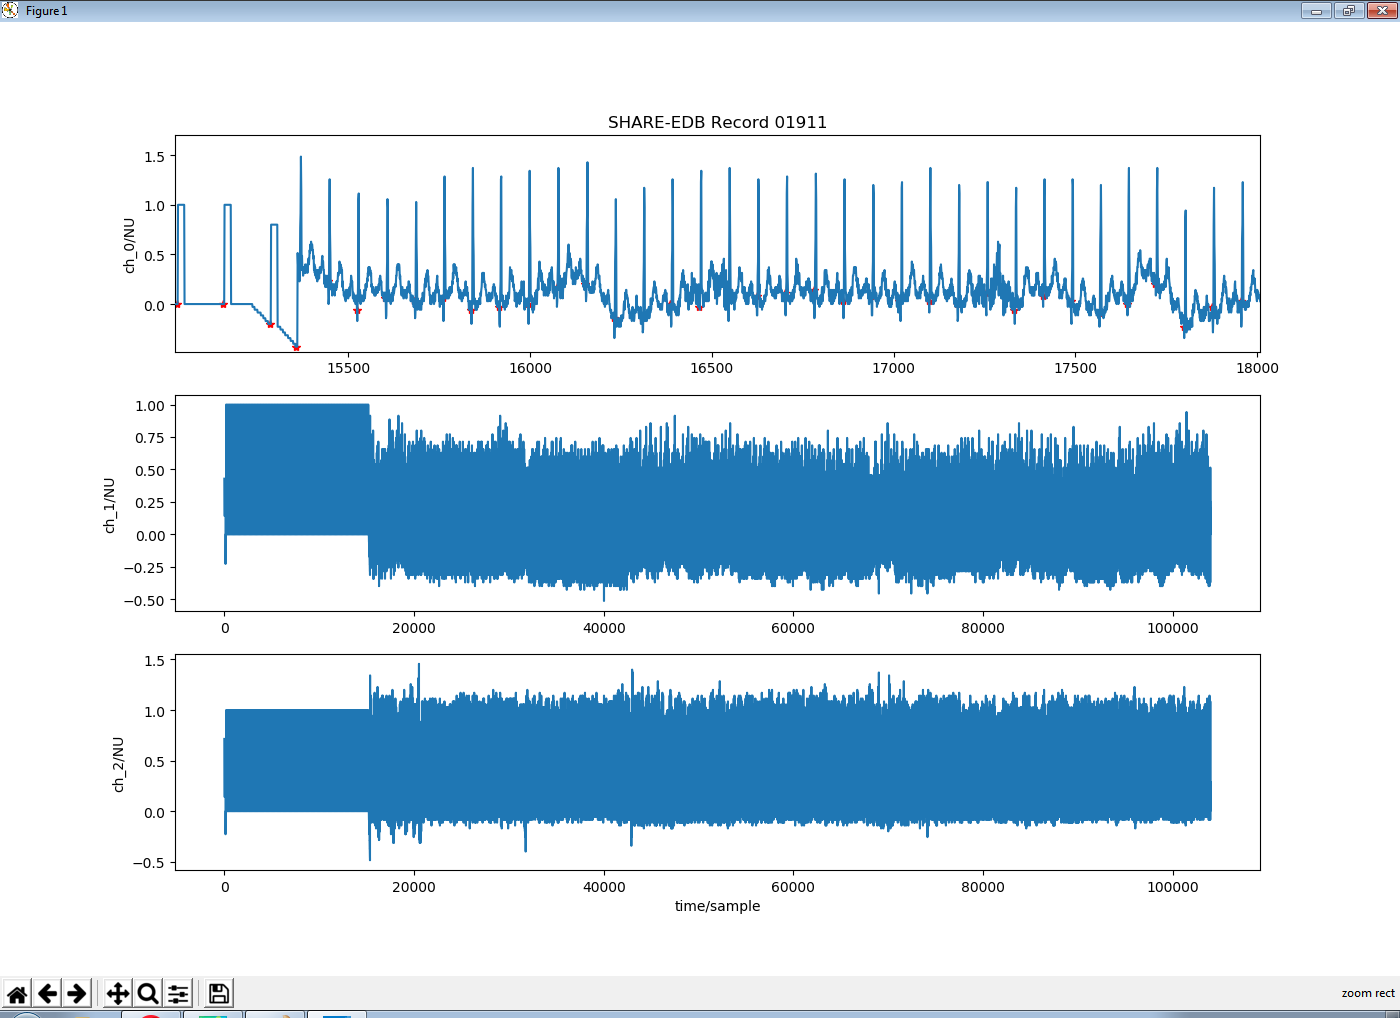
\includegraphics[scale=0.45]{../res/plot-sharee.PNG}
\caption{Prikaz EKG signala iz SHAREE baze podataka koristeći biblioteku \texttt{wfdb}}
\label{plot-hypertension}
\end{figure}

Korištenje \texttt{matplotlib.pyplot.plot} funkcije za prikaz signala demonstrirano je u Listingu \ref{wfdb-pyplot}. Ova funkcija korištena je za kombinovani prikaz signala, kako bi se mogle uočiti razlike u električnom potencijalu i varijacijama između signala iz različitih baza podataka. Odabran je vremenski raspon od 4,000 uzoraka (početni uzorak: br. 100,000, krajnji uzorak: 104,000) van početnog perioda kako bi se izbjegao šum koji nastaje na početku snimanja EKG signala (koji je prisutan u SHAREE signalima). \\

Kombinovani prikaz signala iz dvije ciljane baze podataka vidljiv je na Slici \ref{combined}. Ono što je moguće uočiti na ovom prikazu je razlika između vrijednosti električnog potencijala signala - EKG signal pacijenata koji boluju od aritmije ima mnogo veće varijacije te niži električni potencijal u stanju mirovanja (između otkucaja), dok je kod pacijenata koji boluju od hipertenzije okvirni električni potencijal mnogo viši, te su varijacije vidno manje. Ovu razliku lakše je uočiti na uvećanom grafiku, što je vidljivo na Slici \ref{combined-zoom}. Također je lako uočiti da se otkucaji srca dešavaju mnogo češće na signalu pacijenta koji boluje od hipertenzije.

\begin{figure}
\captionof{lstlisting}{Prikaz EKG signala koristeći biblioteku \texttt{matplotlib.pyplot}}
\label{wfdb-pyplot}
\begin{lstlisting}[language=python]
    # Read arrhythmia signal as a list of samples for plotting

    signal_arrhythmia, fields = wfdb.rdsamp('mitdb/100', channels=[0], sampfrom=100000, sampto=104000)

    # Read hypertension signal as a list of samples for plotting

    signal_hypertension, fields = wfdb.rdsamp('shareedb/01911', channels=[0], sampfrom=100000, sampto=104000)

    # Plot both signals on one plot

    plt.plot(range(4000), signal_arrhythmia, 'b')
    plt.plot(range(4000), signal_hypertension, 'g')

    plt.show()
\end{lstlisting}
\end{figure}

\begin{figure}[H]
\center
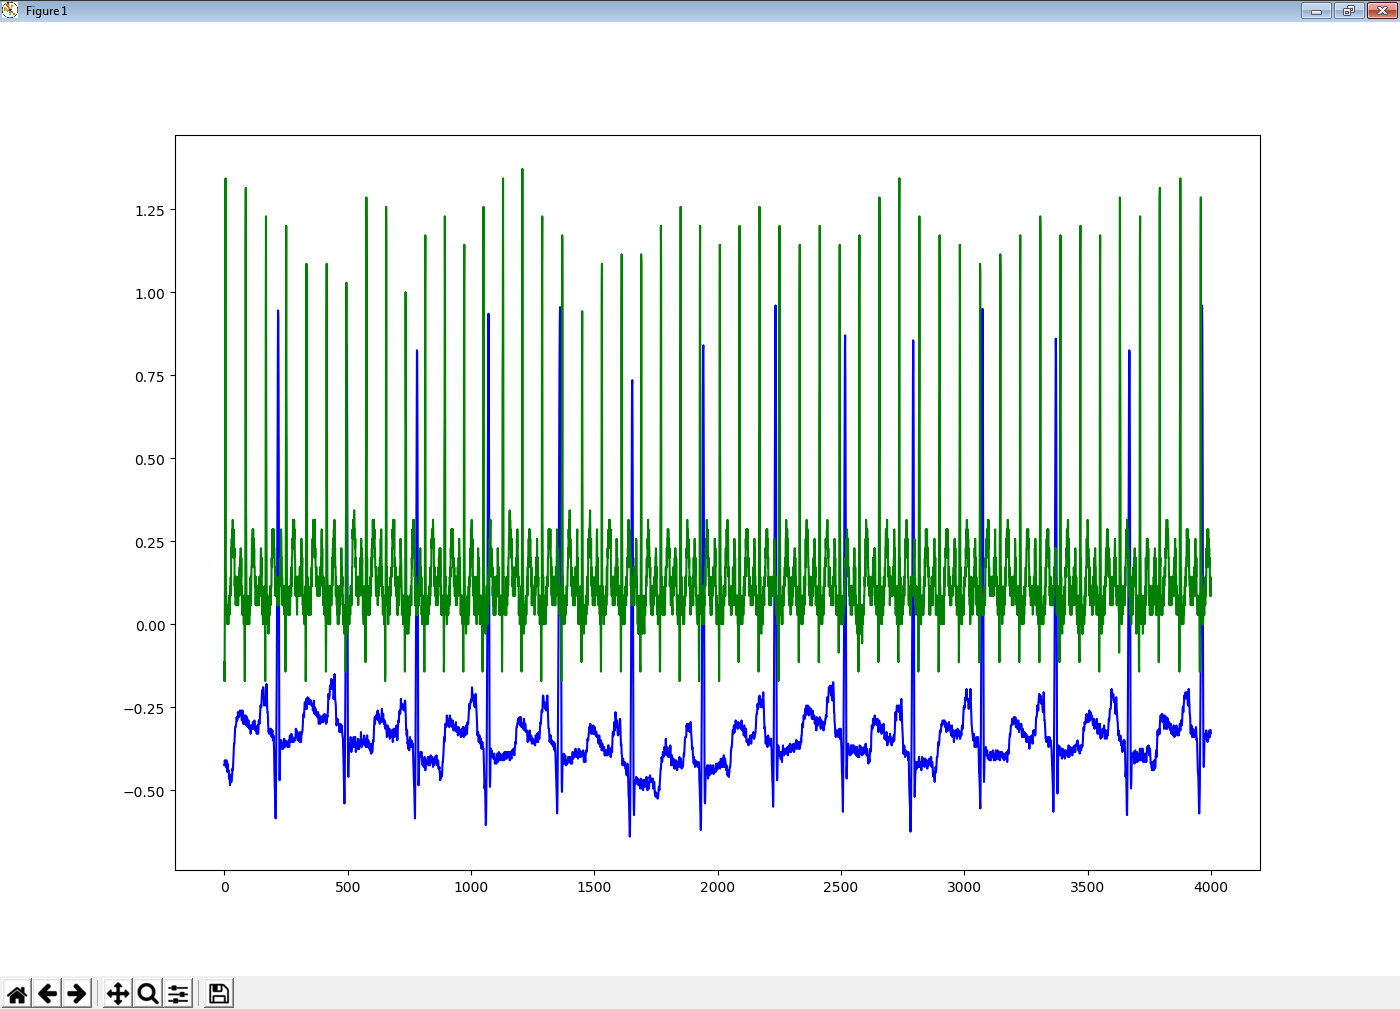
\includegraphics[scale=0.45]{../res/plot-combined.PNG}
\caption{Kombinovani prikaz signala koristeći biblioteku \texttt{matplotlib.pyplot.plot}}
\label{combined}
\end{figure}

\begin{figure}[H]
\center
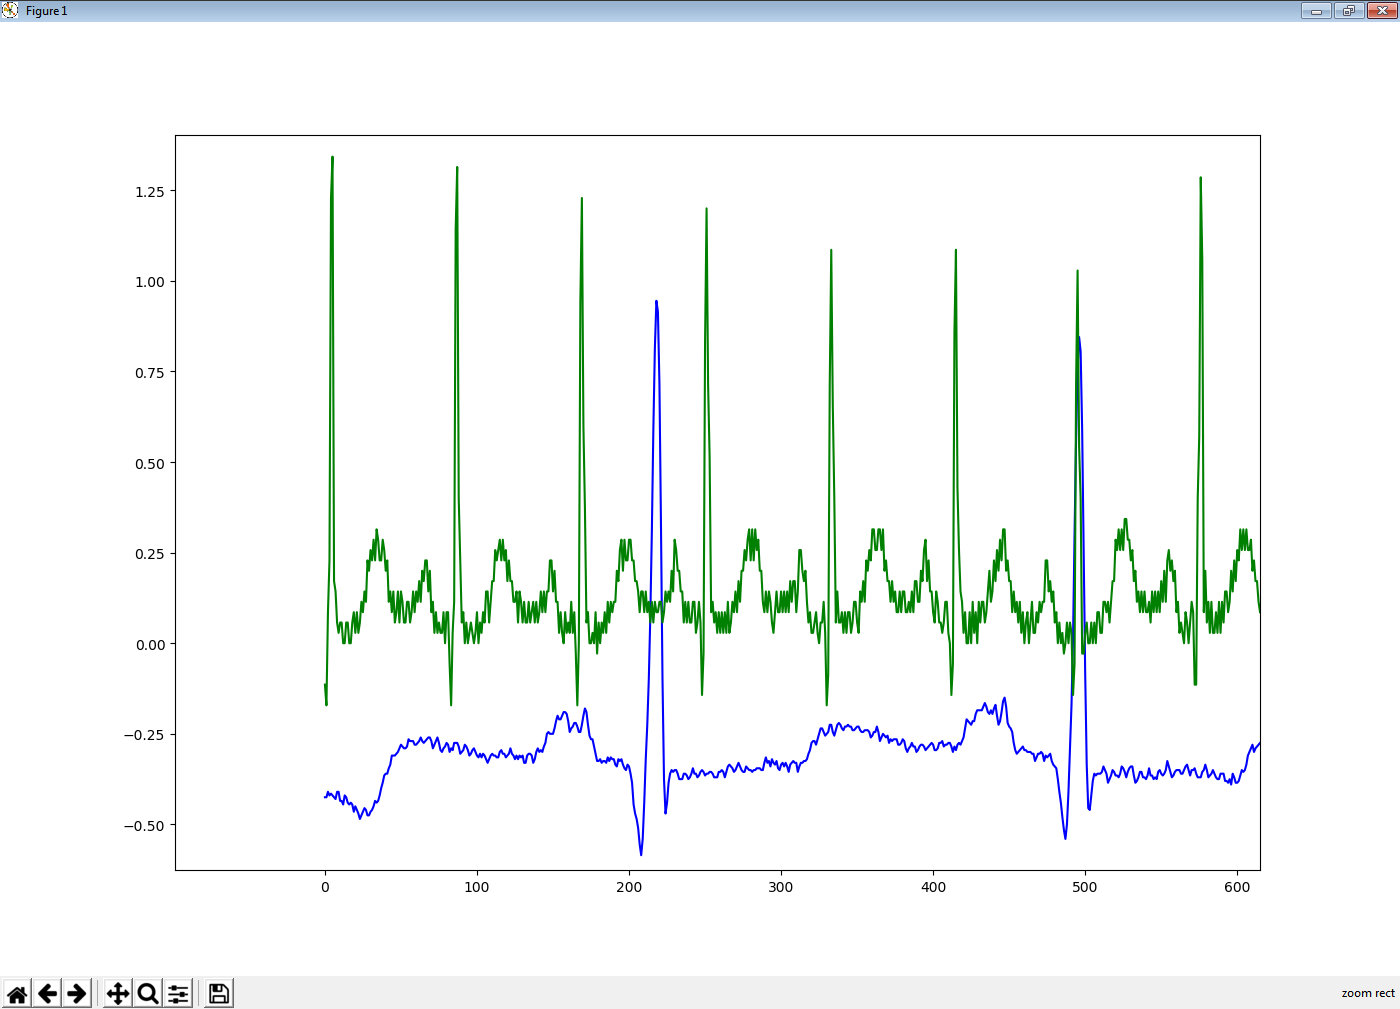
\includegraphics[scale=0.45]{../res/plot-combined-zoom.PNG}
\caption{Uvećani kombinovani prikaz signala koristeći biblioteku \texttt{matplotlib.pyplot.plot}}
\label{combined-zoom}
\end{figure}

\subsection{Analiza otkucaja srca}

\quad Za analizu otkucaja srca koje sadrže EKG signali, prvo je neophodno izvršiti izračun broja otkucaja srca iz električnih potencijala u ovisnosti od vremena (što je inicijalni oblik EKG signala). U tu svrhu koristi se funkcija \texttt{wfdb.processing.compute\_hr}, koja prethodno zahtijeva detekciju QRS kompleksa na signalu, što se čini koristeći funkciju \texttt{wfdb.processing} \texttt{.gqrs\_detect}. Izračunati broj otkucaja srca predstavlja listu sa pojedinačnim brzinama po ciklusu, odnosno, potrebno je izvršiti usrednjavanje ove vrijednosti. U tu svrhu napisana je pomoćna funkcija \texttt{compute\_heart\_rate}. Naposlijetku je izvršeno usrednjavanje svih pojedinačnih vrijednosti otkucaja srca za sve signale u bazi podataka. \\

Ovakav postupak ponovljen je za obje baze podataka, koristeći programski kod prikazan u Listingu \ref{compute-heart-rate}. Dobivena srednja vrijednost brzine otkucaja srca za obje baze te njihova međusobna razlika prikazana je na Slici \ref{heart-rate}, odakle je vidljivo da je ukupna srednja vrijednost brzine otkucaja srca veoma slična za obje baze podataka. No, nije teško doći do zaključka da ovakav način izračuna srednje vrijednosti brzine otkucaja srca ne može puno doprinijeti većim analizama. Iz tog razloga u nastavku će biti izvršena analiza pojedinačnih signala, tj. pojedinačnih brzina otkucaja srca.

\begin{figure}[H]
\captionof{lstlisting}{Izračun pojedinačne i ukupne srednje vrijednosti brzine otkucaja srca za EKG signale jedne baze podataka}
\label{compute-heart-rate}
\begin{lstlisting}[language=python]
 # Iterate through all signals in the arrhythmia database

    for filename in os.listdir(directory_database1):
        if filename.endswith(".dat"):

            record = wfdb.rdrecord('mitdb/' + os.path.splitext(filename)[0], sampfrom=100000, sampto=104000)
            annotation = wfdb.rdann('mitdb/' + os.path.splitext(filename)[0], 'atr', sampfrom=100000, sampto=104000)

            # Detect QRS complex

            qrs_locations = wfdb.processing.gqrs_detect(record.p_signal[:, 0], fs=record.fs)

            # Compute all heart rates for the signal

            heart_rates = wfdb.processing.compute_hr(sig_len=record.sig_len, qrs_inds=qrs_locations, fs=record.fs)

            current_heart_rate = compute_heart_rate(heart_rates)

            overall_heart_rate_arrhythmia += current_heart_rate
            no_of_signals_arrhythmia += 1

            print('Heart rate of the current MIT-BIH signal is: ' + str(current_heart_rate) + ' bpm.')
\end{lstlisting}
\end{figure}

\begin{figure}[H]
\center
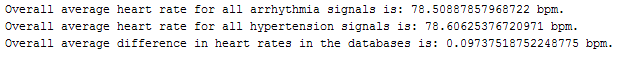
\includegraphics[scale=0.75]{../res/heart-rate-analysis.PNG}
\caption{Prikaz srednje vrijednosti brzine otkucaja srca za obje baze podataka}
\label{heart-rate}
\end{figure}

Za dublje analize korištena je tehnika histogramiranja, odnosno izvršeno je zaokruživanje vrijednosti pojedinačnih brzina otkucaja srca na najbliže vrijednosti te njihov prikaz prema frekvenciji, što je prikazano na Slici \ref{histogram}. Također je korištena i tehnika prikaza dobivenih vrijednosti kao funkcija, kako bi se vidjele fluktuacije u vrijednostima kroz same \textit{dataset}-ove, što je prikazano na Slici \ref{function}. \\

Iz dobivenih prikaza moguće je vidjeti da se frekvencije u brzinama otkucaja srca dosta razlikuju za ciljane baze podataka, te da, kao što je i očekivano, pacijenti koji boluju od hipertenzije mnogo češće imaju tipične vrijednosti krvnog pritiska (opseg 60 - 90 bpm) od pacijenata koji boluju od aritmije, čiji uzorci pokazuju mnogo veće fluktuacije. Iste zaključke moguće je donijeti gledajući prikaz u obliku funkcije, gdje su prelazi u funkciji baze podataka za aritmiju mnogo veći i češći nego kod baze podataka za hipertenziju.

\begin{figure}[H]
\center
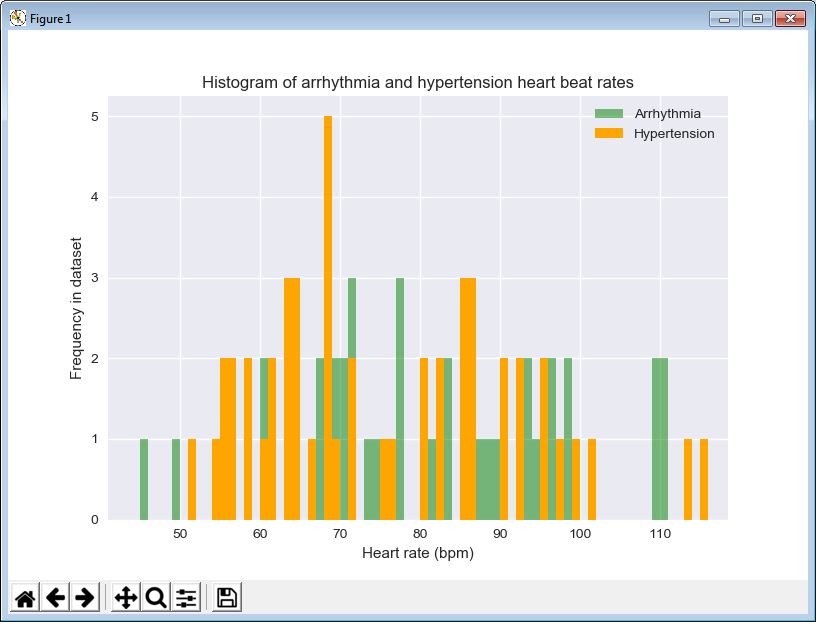
\includegraphics[scale=0.55]{../res/plot-heart-rates-histogram.PNG}
\caption{Prikaz histograma pojedinačnih vrijednosti za otkucaje srca}
\label{histogram}
\end{figure}

\begin{figure}[H]
\center
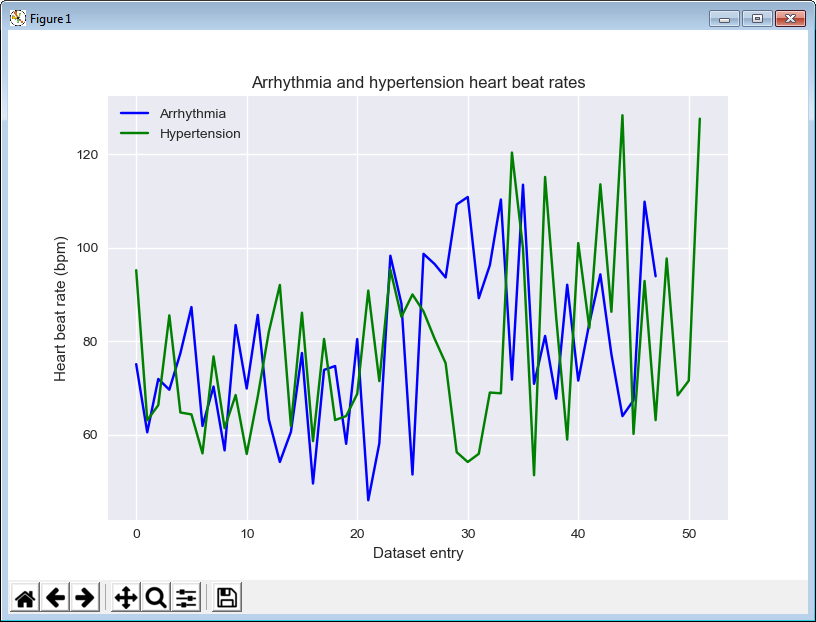
\includegraphics[scale=0.55]{../res/plot-heart-rates.PNG}
\caption{Prikaz funkcija brzina otkucaja srca}
\label{function}
\end{figure}

\subsection{Analiza QRS kompleksa}

\quad Za analizu QRS kompleksa, odnosno varijacije u njihovoj širini, korištena je funkcija \texttt{wfdb} \texttt{.processing.XQRS} u kombinaciji s funkcijom \texttt{xqrs.detect()}. Funkcija \texttt{XQRS} vrši formiranje tačaka koje predstavljaju QRS komplekse, dok funkcija \texttt{detect} vrši detekciju informacija o svim QRS kompleksima koje signal sadrži. Nakon što se detekcija završi, moguće je pročitati informaciju o srednjoj vrijednosti širine QRS kompleksa jednog signala, koristeći funkciju \texttt{qrs\_width}. \\

Samo vršenje detekcije te analize QRS kompleksa izvršeno je za sve signale u obje baze podataka, koristeći programski kod prikazan u Listingu \ref{qrslst}. Nakon toga izvršeno je usrednjavanje vrijednosti te njihova usporedba, kao što je prikazano na Slici \ref{qrs}. Vidljivo je da je razlika u ukupnoj srednjoj širini QRS kompleksa između baza podataka veoma velika, što je i očekivano, budući da su velike fluktuacije u širini QRS kompleksa karakteristika EKG signala pacijenata koji boluju od aritmije.

\begin{figure}[H]
\captionof{lstlisting}{Izračun pojedinačne i ukupne srednje vrijednosti širine QRS kompleksa za EKG signale jedne baze podataka}
\label{qrslst}
\begin{lstlisting}[language=python]
    # Iterate through all signals in the arrhythmia database

    for filename in os.listdir(directory_database1):
        if filename.endswith(".dat"):

            signal, fields = wfdb.rdsamp('mitdb/' + os.path.splitext(filename)[0], channels=[0], sampfrom=100000, sampto=104000)
            ann_ref = wfdb.rdann('mitdb/' + os.path.splitext(filename)[0], 'atr')
            xqrs = wfdb.processing.XQRS(sig=signal[:, 0], fs=fields['fs'])
            xqrs.detect()

            overall_qrs_width_arrhythmia += xqrs.qrs_width
            no_of_signals_arrhythmia += 1
\end{lstlisting}
\end{figure}

\begin{figure}[H]
\center
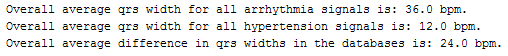
\includegraphics[scale=0.75]{../res/qrs-width.PNG}
\caption{Prikaz srednje vrijednosti širine QRS kompleksa za obje baze podataka}
\label{qrs}
\end{figure}

\newpage

\section{Zaključak}

\quad PhysioNet se sastoji od velikog broja baza podataka EKG signala pacijenata s različitim tipovima kardiovaskularnih bolesti. Analiza ovih podataka može doprinijeti boljem razumijevanju istih bolesti, kao i načina za njihovu ranu detekciju, te samim tim i uspješno liječenje. Iz tog razloga važno je imati širok set alata koji omogućavaju brzu i jednostavnu analizu EKG signala u popularnim programskim jezicima. Glavna prednost \texttt{wfdb} biblioteke je dostupnost, dokumentovanost kao i prilagođenost PhysioNet bazama podataka. \\

Razlike između EKG signala pacijenata koji boluju od aritmije u odnosu na pacijente koji boluju od povišenog krvnog pritiska su očigledne i lako uočljive. Električni potencijal EKG signala pacijenata koji boluju od hipertenzije je viši, brzina otkucaja srca je veća, no srednja vrijednost brzine otkucaja srca približno je ista (i u dozvoljenom opsegu) za obje baze podataka. Pacijenti koji boluju od aritmije češće imaju izrazito velike ili male brzine otkucaja srca (odnosno, izvan tipičnih referentnih vrijednosti), iz kojeg razloga je važno analizirati EKG signale pacijenta te povećati mogućnost dijagnosticiranja aritmije ukoliko je električni potencijal izrazito nizak te fluktuacija od referentnih vrijednosti velika. \\

Možda najveći indikator da osoba boluje od aritmije je svakako širina QRS kompleksa EKG signala. Veoma širok srednji raspon QRS kompleksa ukazuje na to da su razmaci između otkucaja srca veliki, da postoji velika mogućnost od lažne depolarizacije (čime se vrijednost širine QRS kompleksa uduplava) te da QRS kompleksi mnogo odstupaju od referentnih vrijednosti. S druge strane, širina QRS kompleksa nije jak indikator da osoba boluje od hipertenzije - umjesto širine, visina QRS kompleksa mnogo je važnija za analizu kako bi se dijagnosticirala hipertenzija. \\

Svi ovi podaci dobiveni su lako i brzo koristeći biblioteku \texttt{wfdb}. Dobivanje informacija moguće je u roku od nekoliko sekundi (s izuzetkom preuzimanja signala koji se sastoje od velike količine podataka, poput npr. SHAREE signala). Iz tog razloga trebale bi se vršiti analize između više baza podataka, kako bi se potencijalno našče povezanosti između različitih bolesti, njihovog utjecaja na EKG signale pacijenata kako bi se moglo primijeniti mašinsko učenje za automatsku detekciju i dijagnosticiranje različitih stanja na osnovu novoakviziranih EKG signala pacijenata.

\newpage

\bibliographystyle{IEEEtran}
\bibliography{bibliography}

\end{document}